\documentclass{article}

%encoding
%--------------------------------------

%----------------------------
\usepackage{microtype}
\usepackage{fourier}
\usepackage[utf8]{inputenc}
\usepackage[T1]{fontenc}
%units
%--------------------------------------
\usepackage{siunitx}

%drawing
%------------------------------------
\usepackage{tikz} % To generate the plot from csv
\usepackage{pgfplots}
\usepackage{pgfplotstable}
\usepackage{caption}
\usepackage{color, colortbl}
\usepackage{tabularx}

\definecolor{LightCyan}{rgb}{0.88,1,1}
\usetikzlibrary{datavisualization}
\pgfplotsset{compat=newest} % Allows to place the legend below plot
\usepgfplotslibrary{units} % Allows to enter the units nicely

\sisetup{
  round-mode          = places,
  round-precision     = 2,
}



\usetikzlibrary{arrows, positioning, calc, datavisualization}

\pgfplotsset{
  standard/.style={
    axis x line=bottom,
    axis y line=middle,
  }
}
\begin{document}
%\begin{luacode*}
function string:split(sep)
        local sep, fields = sep or "%s", {}
        local pattern = string.format("([^%s]+)", sep)
        self:gsub(pattern, function(c) fields[#fields+1] = c end)
        return fields
end

function printHyperbola()
    local lines={}

    for line in io.lines("dampf.csv") do
            table.insert(lines, line)
    end
    tex.sprint("\\addplot[color=black] coordinates{")

    for i=2,#lines do
        local a=lines[i]:split()
        tex.sprint("("..a[1]..","..a[2]..")")
    end
     tex.sprint("};")
    tex.sprint("\\addplot[color=blue] coordinates{")

    for i=2,#lines do
        local a=lines[i]:split()
        tex.sprint("("..a[1]..","..a[3]..")")
    end
     tex.sprint("};")

end
\end{luacode*}
%\begin{figure}
\centering
     \begin{tikzpicture}
            \begin{axis}[standard,xlabel=Temperatur,ylabel=Druck]
                \directlua{printHyperbola()}
            \end{axis}
        \end{tikzpicture}
     \end{figure}

\noindent
\section{Ziel des Versuches}
Der Versuch soll den Studenten an das Prinzip der Rektifikation heranführen, indem ein
vorgegebenes Toluol-Methylcyclohexan-Gemisch mittels verschiedener Kolonnen getrennt
werden soll. Dabei soll die theoretische Bodenzahl bestimmt werden, bei einer
Bodenkolonne unter Variation der Heizlast und bei einer Packungskolonne unter Variation
des Rücklaufverhältnises.
\section{Versuchsdurchführung}
Zu Beginn des Versuches wurde den bereits laufenden Kolonnen je eine Probe entnommen
und mittels eines Refraktometers die Zusammensetzung bestimmt. Nach der Entnahme wird
die Heizlast, beziehungsweise das Rücklaufverhältnis variiert. Nach einer geeigneten Dauer
zum Einstellen des Gleichgewichts wird abermals eine Probe entnommen. Dies wird
insgesamt viermal wiederholt.
\section{Messwerte}
% subsection subsection_name (end)
\begin{table}[ht!]
  \centering
 \begin{tabularx}{\textwidth}{XXXX}
Heizlast & $n^{20}_D$ & $x_{Kopf}$ &  $T^{Kopf}$  \\
\hline
\rowcolor{LightCyan}
220 V & 1.4750 & 0.43 &  104.1 \si\celsius    \\
185 V & 1.4750 & 0.44 &  103.9 \si\celsius    \\
170 V & 1.4740 & 0.46 &  103.6 \si\celsius    \\
145 V & 1.4739 & 0.48 &  103.2 \si\celsius    \\
\end{tabularx}
  \caption{Messwerte der Bodenkolonne}

\end{table}

\begin{table}[ht!]
  \centering
 \begin{tabularx}{\textwidth}{XXX}
Rücklaufverhältnis & $n^{20}_D$  & $x$  \\
\hline
\rowcolor{LightCyan}
3 & 1.4860 &  0.16167   \\
5  & 1.4851 &   0.17234   \\
\rowcolor{LightCyan}
10  & 1.4855 &  0.16700   \\
$\infty$  & 1.4860 &  0.16167  \\
\end{tabularx}
  \caption{Messwerte der Packungskolonne}
\end{table}

\section{Auswertung}
\subsection{Siedediagramm}
\begin{figure}
  \begin{center}

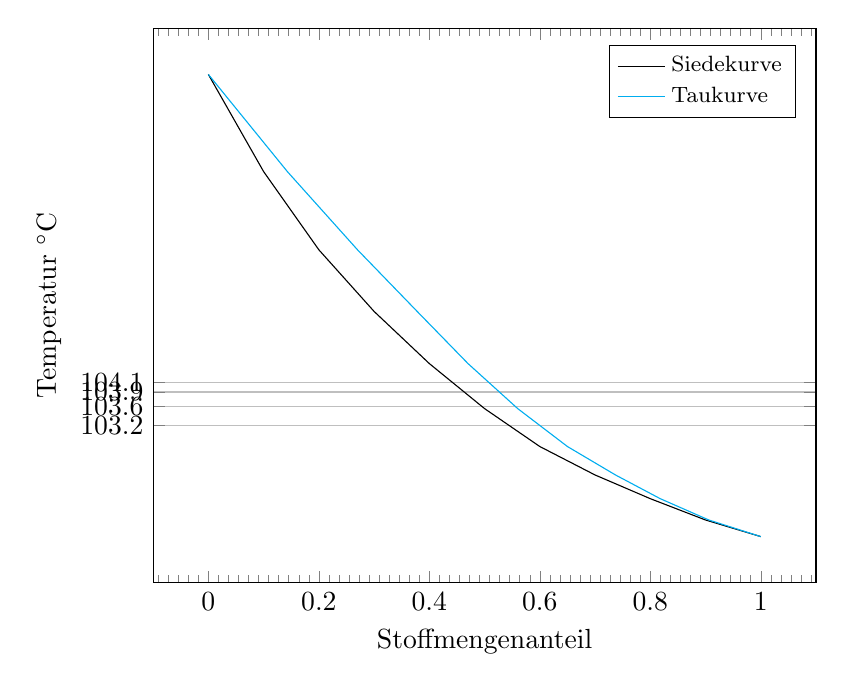
\begin{tikzpicture}
    \pgfplotsset{width=10cm,
        compat=1.3,
        legend style={font=\footnotesize}}
    \begin{axis}[
    xlabel={Stoffmengenanteil},
    ylabel={Temperatur \si\celsius},
    ytick={104.1, 103.9, 103.6, 103.2},
   minor tick num=10,
    ymajorgrids=true,
    legend cell align=left,
    legend pos=north east]
    \addplot[color=black] table{
         0.00 110.60
         0.10 108.55
         0.20 106.90
         0.30 105.60
         0.40 104.50
         0.50 103.55
         0.60 102.75
         0.70 102.15
         0.80 101.65
         0.90 101.20
         1.00 100.85
    };
  \addplot[color=cyan] table{
         0.000 110.60
         0.143 108.55
         0.270 106.90
         0.378 105.60
         0.470 104.50
         0.560 103.55
         0.650 102.75
         0.737 102.15
         0.818 101.65
         0.906 101.20
         1.000 100.85
};

    \addlegendentry{Siedekurve}
    \addlegendentry{Taukurve}

     \end{axis}

    \end{tikzpicture}
\end{center}
\caption{Siedediagramm}
\end{figure}

\subsection{Ermittlung der Kopfzusammensetzung} % (fold)

\begin{table}[ht!]
  \centering
 \begin{tabularx}{\textwidth}{XXXX}
Heizlast \si{\volt} & $T_{Kopf}$ & $x_D$ & $y_D$  \\
\hline
\rowcolor{LightCyan}
145 & 106.9 & 0.2029 &  0.2680    \\
170 & 106.2 & 0.2519 &  0.3237 \\
\rowcolor{LightCyan}
185 & 104.4 & 0.4042 &  0.4041 \\
220 & 102.4 & 0.6581 &  0.6986 \\
\end{tabularx}
  \caption{Zusammensetzung des Destillats in der Bodenkolonne}
\end{table}

\begin{table}[ht!]
  \centering
 \begin{tabularx}{\textwidth}{XXXX}
Rücklaufverhältnis & $T_{Kopf}$ & $x_D$ & $y_D$  \\
\hline
\rowcolor{LightCyan}
3         & 104.1  &  0.4347 & 0.5093   \\
5         & 103.9  &  0.4562 & 0.5291   \\
\rowcolor{LightCyan}
10        & 103.6  &  0.4903 & 0.5597   \\
$\infty$  & 103.2  &  0.5401 & 0.6026  \\
\end{tabularx}
  \caption{Zusammensetzung des Destillats in der Packungskolonne}
\end{table}



\begin{equation}
y = -5.64 x ^ 3 + 17.14 x ^2 - 21.22 x + 110.55
\qquad \text{Taukurve}
\end{equation}

\begin{equation}
y = 2.54 x ^ 3 + 2.34 x ^2 - 14.61 x + 110.60
\qquad \text{Siedekurve}
\end{equation}
% subsection ermittlung_der_kopfzusammensetzung_ (end)


\subsection{Ermittlung der Blasenzusammensetzung} % (fold)
Zur Erstellung einer Kalibrierkurve, für die Abhängigkeit des Brechungsindex‘ von der
Blasenzusammensetzung, muss zuerst der Molenbruch $x_{MCH}$
des Leichtsieders nach Formel (3) berechnet werden:
\begin{equation}
  x_{MCH} = \frac{n_{MCH}}{n_{MCH}+n_{Tol}} = \frac{\frac{\rho \cdot V_{MCH}}{M_{MCH}}}{\frac{\rho _{MCH} \cdot V_{MCH}}{M_{MCH}}+\frac{\rho _{Tol} \cdot V_{Tol}}{M_{Tol}}}
\end{equation}
Daraus folgen die Werte zur Erstellung der Kalibrierkurve:
\begin{table}[ht!]
  \centering
 \begin{tabularx}{\textwidth}{XXXX}
$V_{MCH}$ \si{\cubic\centi\meter} & $V_{Tol}$ \si{\cubic\centi\meter}  & $n_{D^{20}}$ & $x_{MCH}$  \\
\hline
\rowcolor{LightCyan}
0  & 50& 1.49736 & 0.0000\\
5  & 45& 1.48948 & 0.0847\\
\rowcolor{LightCyan}
10 & 40& 1.48163 & 0.1723\\
15 & 35& 1.47401 & 0.2631\\
\rowcolor{LightCyan}
20 & 30& 1.46608 & 0.3570\\
25 & 25& 1.45884 & 0.4544\\
\rowcolor{LightCyan}
30 & 20& 1.45146 & 0.5554\\
35 & 15& 1.44432 & 0.6603\\
\rowcolor{LightCyan}
40 & 10& 1.43702 & 0.7691\\
45 & 5 & 1.42969 & 0.8823\\
\rowcolor{LightCyan}
50 & 0 & 1.42312 & 1.0000\\
\end{tabularx}
  \caption{Zusammensetzung des Destillats in der Packungskolonne}
\end{table}
Die zugehörige Regressionsgerade lautet:
\begin{equation}
  y = 0.019 x^2 -0.093 x + 1.4972
   \qquad \text{$R^2$=1}
\end{equation}
Setzt man die Regressionsgerade (4) mit den gemessenen Brechungsindizes gleich, so lassen
sich die Sumpfzusammensetzungen für die Boden- und die Packungskolonne bestimmen.
Der gemittelte Brechungsindex für die Bodenkolonne beträgt $n_{D^{20}}$
, für diesen ergibt sich eine Sumpfzusammensetzung von. Für die Packungskolonne, mit
einem gemittelten Brechungsindex von ergibt sich eine Sumpfzusammensetzung von.

\begin{figure}[htbp!]
      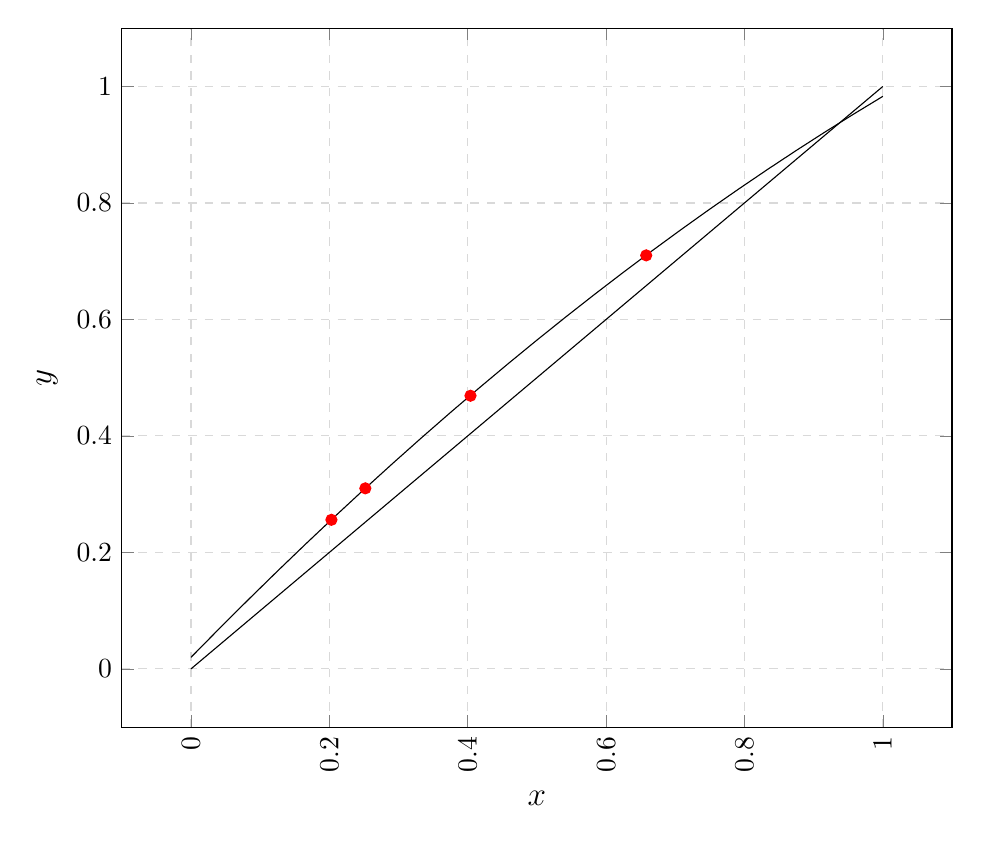
\begin{tikzpicture}
      \begin{axis}[
          width=\linewidth, % Scale the plot to \linewidth
          grid=major,
          grid style={dashed,gray!30},
          xlabel= $x$, % Set the labels
          ylabel= $y$,
          xlabel style={font=\large},
          ylabel style={font=\large},
          %x unit= \si{\milli\volt} , % Set the respective units
          %y unit= \si{\volt},
          x tick label style={rotate=90,anchor=east}
          ]


\addplot[only marks,color=red] table{
   X Y
   0.203 0.256
   0.252 0.310
   0.404 0.469
   0.658 0.710
};

\addplot[domain=0:1]{x};

\addplot[domain=0:1]{-0.25221*x^(2)+1.21531*x+0.0199};

%\addlegendentry{ }
\end{axis}
\end{tikzpicture}
\caption*{Abbildung 1.1: Gleichgewichtsdiagramm  McCabe Bodenkolonne}

\end{figure}

\begin{figure}[htbp!]
      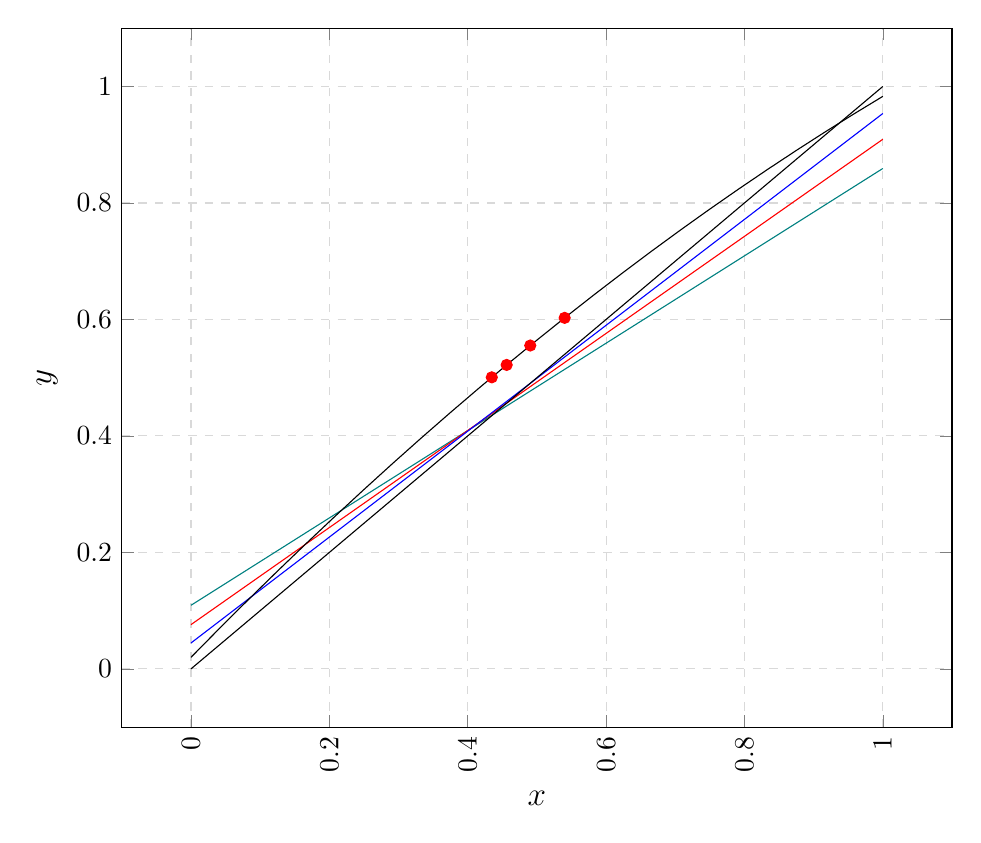
\begin{tikzpicture}
      \begin{axis}[
          width=\linewidth, % Scale the plot to \linewidth
          grid=major,
          grid style={dashed,gray!30},
          xlabel= $x$, % Set the labels
          ylabel= $y$,
          xlabel style={font=\large},
          ylabel style={font=\large},
          %x unit= \si{\milli\volt} , % Set the respective units
          %y unit= \si{\volt},
          x tick label style={rotate=90,anchor=east}
          ]


\addplot[only marks,color=red] table{
   X Y
0.43478 0.50061
0.45627 0.52190
0.49041 0.55524
0.54009 0.60270
};

\addplot[domain=0:1,color=teal]{3/4*x+0.1092};
\addplot[domain=0:1,color=red]{5/6*x+0.076};
\addplot[domain=0:1,color=blue]{10/11*x+0.0445};

\addplot[domain=0:1]{x};
\addplot[domain=0:1]{-0.25221*x^(2)+1.21531*x+0.0199};

%\addlegendentry{ }
\end{axis}
\end{tikzpicture}
\caption*{Abbildung 1.2: McCabe Füllkörperkolonne }

\end{figure}


\end{document}
